%   ===================================================
%	Plot the Consumer surplus, producer surplus, and deadweight loss
%	following a price floor.

%	Coordinates are computed automatically based on the arbitrary demand
%	and supply functions provided by the user, and the price floor.

%	Author: Patrick Blanchenay
%   ===================================================

\documentclass{standalone}
% =============================================
\usepackage{tikz}               % to draw things
\usepackage{pgfplots}           % to draw plots & curves
\pgfplotsset{compat=1.8}
\usetikzlibrary{calc,intersections,arrows}  % to find and define intersections of curves, equilibria...
\usepgfplotslibrary{fillbetween} % to shade areas
% ---------------------------------------------------------------------
% Coordinate extraction % https://tex.stackexchange.com/questions/420498/extract-convert-store-and-reuse-x-y-coordinate-components/426245#426245
% #1: node name
% #2: output macro name: x coordinate
% #3: output macro name: y coordinate
\newcommand{\Getxycoords}[3]{%
	\pgfplotsextra{%
		% using `\pgfplotspointgetcoordinates' stores the (axis)
		% coordinates in `data point' which then can be called by
		% `\pgfkeysvalueof' or `\pgfkeysgetvalue'
		\pgfplotspointgetcoordinates{(#1)}%
		% `\global' (a TeX macro and not a TikZ/PGFPlots one) allows to
		% store the values globally
		\global\pgfkeysgetvalue{/data point/x}{#2}%
		\global\pgfkeysgetvalue{/data point/y}{#3}%
	}%
}
\tikzset{ % to make dots on the graph
dot/.style = {circle, fill, minimum size=#1,
           inner sep=0pt, outer sep=0pt},
dot/.default = 6pt % size of the circle diameter 
}
% =============================================
\begin{document}

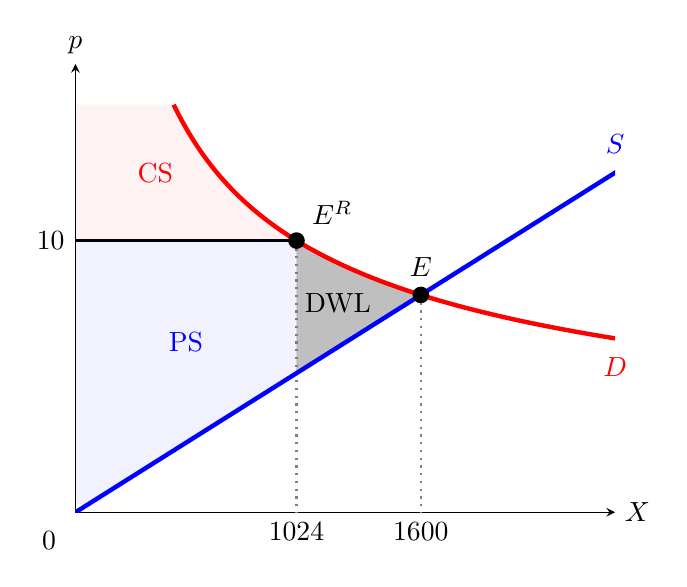
\begin{tikzpicture}[
% ========= Things to change ======================
   	declare function={
   		demandfunction(\p)     =   102400*(\p)^(-2);      % Demand
   		inversedemand(\x)      =   320/sqrt(\x);    		% Inverse demand (calculate manually)
   		supplyfunction(\p)      =   200*\p;					% Supply
   		inversesupply(\x)		=   \x / 200;				% Inberse supply
   	}] % 

 % Graph settings
\def\pmax{15}				% Maximum price to display on the vertical axis
\def\pmin{0}   
\def\qmax{2500}				% Maximum quantity supply for the industry
\def\qmin{0}				% Minimum quantity supply for the industry
\def\pricefloor{10} 			% PRICE FLOOR

 
% ======= GRAPH HAPPENS HERE =========== 
\begin{axis}[  
     	axis lines=middle, xlabel style={right }, ylabel style={above },
     	xlabel=$X$, ylabel=$p$, 
     	xmin=\qmin,xmax=\qmax, % quantities
     	ymin=\pmin,ymax=\pmax, % price
     	restrict y to domain=\pmin:\pmax,
     	xtick={\empty},
     	ytick=\empty,
%            axis x discontinuity=parallel,
		enlarge y limits={upper=0.15},
% 		enlarge x limits={upper=0.5},
		clip mode=individual,
     	]
% ====================================
% Axes origin & axes
% ====================================
\node [label=-135:$0$] (origin) at (axis cs:\qmin,\pmin) {};	
\coordinate (verticalaxis) at (axis cs:\qmin,\pmax); 
\coordinate (horizontalaxis) at (axis cs:\qmax,\pmin); 
\path[name path=vertaxis] (axis cs:0,0) -- (axis cs:0,\pmax); % Needed for shading     	
     	
%  Demand path (not drawn,  just used to find the intersection)
\addplot[name path global=demand,samples=100,draw=none,domain=1.4:\pmax,variable=p] 
	          	(demandfunction(p),p) ; 
% Supply path (not drawn,  just used to find the intersection)
\addplot[name path global=supply,samples=10,draw=none,domain=\pmin:\pmax,variable=p] 
         	 	(supplyfunction(p),p) ;    
   
% Useful nodes for shading etc.
\coordinate (demandmax) at  (axis cs:{demandfunction(\pmax)},\pmax); %
\coordinate (demandmaxvertaxis) at  (demandmax -| verticalaxis); %

% ====================================
% Equilibrium without price floor, 
% and get coordinates in print-friendly format
% ====================================
\path [name intersections={of=supply and demand,by=LROriginalEquil}];  
\Getxycoords{LROriginalEquil}{\Ex}{\Ey}
\def\originalqtty{\pgfmathprintnumber[ precision=0, set thousands separator={}]{\Ex}} % Can adjust precision if qtty is not integer
\def\originalprice{\pgfmathprintnumber[fixed, precision=0]{\Ey}} % Can adjust precision if price is not integer

\draw[thick,gray,dotted]  (LROriginalEquil) -- (LROriginalEquil |- horizontalaxis) node[below,black] {$\originalqtty$}  ; % Label quantity

% ====================================
% Equilibrium WITH price floor, 
% and get coordinates in print-friendly format
% ====================================     			
% Demand point under price floor	
\coordinate (restricteddemand) at (axis cs:{demandfunction(\pricefloor)},\pricefloor); %  demand	 under price restriction
\coordinate (restricteddemandaxis) at (restricteddemand -| verticalaxis); %
% Compute quantity under price floor
\pgfkeys{/pgf/fpu}
\pgfmathsetmacro{\restrictedqttynb}{demandfunction(\pricefloor)}
\pgfkeys{/pgf/fpu=false}
\def\restrictedqtty{\pgfmathprintnumber[ precision=0, set thousands separator={}]{\restrictedqttynb}} % Can adjust precision if qtty is not integer

% Supply point under price floor
\coordinate (restrictedsupply) at (axis cs:{demandfunction(\pricefloor)},{inversesupply(demandfunction(\pricefloor))}); %  supply	 under price restriction
			
% Label restricted quantity (and price floor)
\draw[thick,gray,dotted]  (restricteddemand) -- (restricteddemand |- horizontalaxis) node[below,black] {$\restrictedqtty$}  ;
\draw[very thick,black,solid]  (restricteddemand) -- (restricteddemand -| verticalaxis) node[left,black] {$\pricefloor$}  ;

% ====================================
% CONSUMER SURPLUS AREA
% ====================================
\addplot [ fill=red,  fill opacity=0.05   ]
    fill between[
        of=demand and vertaxis,
        soft clip={domain y=\pricefloor:\pmax},
    ];
\node[red] at (barycentric cs:restricteddemand=1,restricteddemandaxis=1,demandmax=1,demandmaxvertaxis=1)  {CS};  % Label in middle of area

% ====================================
% PRODUCER SURPLUS AREA
% ====================================
\draw[fill=blue,draw=none,  fill opacity=0.05] 
	(origin) -- (restricteddemand -| verticalaxis) -- (restricteddemand) -- (restrictedsupply) -- (origin);
\node[blue] at (barycentric cs:restricteddemand=1,restrictedsupply=1,restricteddemandaxis=1,origin=1)  {PS};  % Label in middle of area

% ====================================
% DEADWEIGHT LOSS AREA
% ====================================
\addplot [
        fill=gray, 
        fill opacity=0.5
    ]
    fill between[
        of=demand and supply,
        soft clip={domain=\restrictedqttynb:\Ex},
    ];
\node at (barycentric cs:LROriginalEquil=1  ,restricteddemand=1 ,restrictedsupply=1)  {DWL};    % Label in middle of area 

% ====================================
% Lastly, DRAW demand and supply, and the dots
% ====================================
\addplot[samples=100,red, ultra thick,domain=\pmax:6,variable=p] 
          	(demandfunction(p),p) ; 
\node[label={[red]-90:$D$}] at (axis cs:\qmax,{inversedemand(\qmax)}) {};
% Supply
\addplot[samples=10,blue, ultra thick,domain=\pmin:\pmax,variable=p] 
         	 	(supplyfunction(p),p) ; 
\node[label={[blue]90:$S$}] at (axis cs:\qmax,{inversesupply(\qmax)}) {};
\node[dot,fill,label=90:$E$]  at (LROriginalEquil) {};
\node[dot,fill,label=above right:$E^R$]  at (restricteddemand) {};

     
\end{axis}

\end{tikzpicture}


%NB: the equilibrium without price restriction is indicated as $E$. The equilibrium with price restriction is indicated as $E^R$.

% =============================================	
\end{document}